% sections/class1.tex

\section{Class 1, Early Developments}
\subsection{BCG Experience Curve}
Cost falls as cumulative output increases until a plateau.
\textbf{Strategy:} Plan production/investments to gain competitive cost advantage.

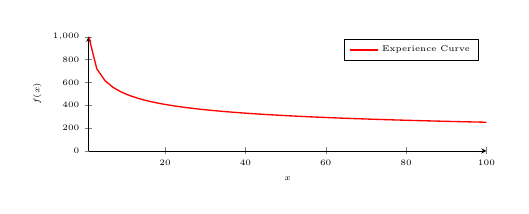
\begin{tikzpicture}[scale=0.6, transform shape]
    \begin{axis}[
            width=10cm, height=4cm,
            axis lines = left,
            xlabel = {\(x\)},
            ylabel = {\(f(x)\)},
            ymin=0, ymax=1000,
            tick label style={font=\tiny},
            label style={font=\tiny}
        ]
        \addplot [
            domain=1:100,
            samples=50,
            color=red, thick
        ]
        {1000*x^(-0.3)};
        \addlegendentry{\tiny Experience Curve}
    \end{axis}
\end{tikzpicture}

\subsection{Functional vs. Divisional Structure}
\textbf{Functional:} Grouped by job roles (Mkt, Fin). Best for stable/single product
lines. \\
\textbf{Divisional:} Grouped by product/market. Responsive but resource-redundant.

\textbf{Strategy:} Choose structure based on product complexity and market dynamics.
Divisional for diverse/fast-changing markets, functional for
stable/single-product firms. Allows focus on core competencies and efficient
resource use.

\begin{tikzpicture}[
        font=\tiny\sffamily,
        >=Latex,
        node distance=3mm and 4mm,
        box/.style={draw, rounded corners=1pt, align=center, minimum width=10mm, minimum height=5mm, fill=white},
        smallbox/.style={draw, rounded corners=1pt, align=center, minimum width=15mm, minimum height=4mm, fill=white},
        comment/.style={draw, align=left, text width=30mm, rounded corners=1pt, fill=gray!5},
        dashedarrow/.style={-{Latex}, dashed},
        scale=1, transform shape
    ]

    % === Functional Structure ===
    \node[box, fill=blue!10] (ceof) {CEO (Functional)};

    \node[box, below left=4mm and 5mm of ceof] (mktf) {Marketing};
    \node[box, below right=4mm and 5mm of ceof] (opsf) {Operations};
    \node[box, below=4mm of ceof] (finf) {Finance};

    \draw[->] (ceof) -- (mktf);
    \draw[->] (ceof) -- (finf);
    \draw[->] (ceof) -- (opsf);

    \node[smallbox, below=2mm of mktf] (pa_m) {Prod A Mkt};
    \node[smallbox, below=1mm of pa_m] (pb_m) {Prod B Mkt};
    \draw[->] (mktf) -- (pa_m); \draw[->] (pa_m) -- (pb_m);

    \node[smallbox, below=2mm of finf] (pa_f) {Prod A Fin};
    \node[smallbox, below=1mm of pa_f] (pb_f) {Prod B Fin};
    \draw[->] (finf) -- (pa_f); \draw[->] (pa_f) -- (pb_f);

    \node[smallbox, below=2mm of opsf] (pa_o) {Prod A Ops};
    \node[smallbox, below=1mm of pa_o] (pb_o) {Prod B Ops};
    \draw[->] (opsf) -- (pa_o); \draw[->] (pa_o) -- (pb_o);

    \begin{pgfonlayer}{background}
        \node[draw=blue!70, fill=blue!5, fit=(ceof) (pb_m) (pb_o), inner sep=2pt, label={[yshift=-2pt]above:\textbf{Functional}}] (funcbox) {};
    \end{pgfonlayer}

    % === Divisional Structure ===
    \node[box, fill=green!10, right=32mm of ceof] (ceod) {CEO (Divisional)};

    \node[box, fill=yellow!20, below left=4mm and -5mm of ceod] (diva) {Div A (Prod A)};
    \node[box, fill=yellow!20, below right=4mm and -5mm of ceod] (divb) {Div B (Prod B)};

    \draw[->] (ceod) -- (diva);
    \draw[->] (ceod) -- (divb);

    \node[smallbox, below=2mm of diva] (mktga) {Mkt / Fin};
    \node[smallbox, below=1mm of mktga] (opsa) {Ops / HR};
    \draw[->] (diva) -- (mktga); \draw[->] (mktga) -- (opsa);

    \node[smallbox, below=2mm of divb] (mktgb) {Mkt / Fin};
    \node[smallbox, below=1mm of mktgb] (opsb) {Ops / HR};
    \draw[->] (divb) -- (mktgb); \draw[->] (mktgb) -- (opsb);

    \begin{pgfonlayer}{background}
        \node[draw=green!70, fill=green!5, fit=(ceod) (opsa) (opsb), inner sep=2pt, label={[yshift=-2pt]above:\textbf{Divisional}}] (divbox) {};
    \end{pgfonlayer}

\end{tikzpicture}

\subsection{BCG Growth Matrix}
\textbf{Stars:} High market share/growth. Invest to maintain. \\
\textbf{Dogs:} Low share/growth. Divest or niche focus. \\
\textbf{Question Marks:} Low share/high growth. Invest to grow or divest. \\
\textbf{Cash Cows:} High share/low growth. Milk profits, minimal investment.

\begin{center}
    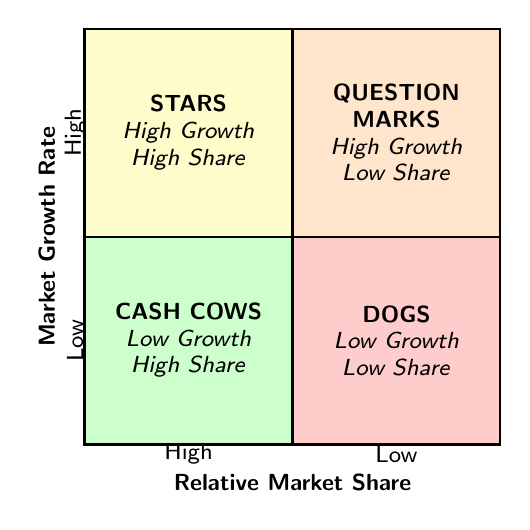
\begin{tikzpicture}[
            scale=1.2, transform shape,
            font=\sffamily\scriptsize,
            box/.style={minimum size=2.2cm, draw, thick, align=center}
        ]
        % The Grid
        \node[box, fill=yellow!20] (stars) at (0,2.2) {\textbf{STARS} \\ \textit{High Growth} \\ \textit{High Share}}; \node[box, fill=orange!20] (question) at (2.2,2.2) {\textbf{QUESTION} \\ \textbf{MARKS} \\ \textit{High Growth} \\ \textit{Low Share}}; \node[box, fill=green!20] (cash) at (0,0) {\textbf{CASH COWS} \\ \textit{Low Growth} \\ \textit{High Share}}; \node[box, fill=red!20] (dogs) at (2.2,0) {\textbf{DOGS} \\ \textit{Low Growth} \\ \textit{Low Share}};

        % Axis Labels (Y-axis: Market Growth)
        \node[rotate=90] at (-1.5,1.1) {\textbf{Market Growth Rate}}; \node[rotate=90] at (-1.2,2.2) {High}; \node[rotate=90]
        at (-1.2,0) {Low};

        % Axis Labels (X-axis: Market Share)
        \node at (1.1,-1.5) {\textbf{Relative Market Share}}; \node at (0,-1.2) {High}; \node at (2.2,-1.2) {Low};

    \end{tikzpicture}
\end{center}

\textbf{Strategy:} Allocate resources based on quadrant. Invest in Stars/Question
Marks, milk Cash Cows, divest Dogs. Regularly reassess as market conditions
change.

\section{Case 1: US Airlines vs. Starbucks}
\textbf{Airlines (Commodity/Cost):} High fixed costs, price-sensitive demand, and
``razor-thin'' margins. Post-1978 deregulation led to \textbf{Hub-and-Spoke} systems to drive efficiency and regional dominance.
\textbf{Starbucks (Differentiation):} Focused on the ``Third Place'' experience and
emotional connection. Uses store clustering for visibility and treats employees
as ``partners'' to maintain service quality.

\subsubsection{Comparative Performance (2014)}
\begin{center}
    \scriptsize
    \begin{tabular}{@{}lll@{}}
        \toprule
        \textbf{Metric} & \textbf{Airlines (American)} & \textbf{Starbucks} \\ \midrule Revenue & $\$42.6$ Billion & $\$16.45$ Billion \\ Net
        Margin          & $\sim 10\%$                  & $\mathbf{12.6\%}$  \\ Op. Income & $\$2.316$ Billion &
        $\$3.081$ Billion                                                   \\ Market Share & $16.9\%$ (Southwest – RPM) & $26.1\%$
        (Premium Roast)                                                     \\ \bottomrule
    \end{tabular}
\end{center}

\subsubsection{Key Strategic Drivers}
\begin{itemize}
    \item \textbf{Airlines (Cost Leadership):} Advantage via \textbf{Load Factors} and minimizing Cost per Available Seat Mile (CASM). Loyalty is
          primarily structural (Frequent Flyer miles) rather than brand-based.
    \item \textbf{Starbucks (Differentiation):} Advantage via \textbf{Customer Experience}. Pricing power is maintained by selling an environment,
          not just coffee.
    \item \textbf{Cost Management:} Airlines hedge volatile fuel costs and manage rigid labor
          unions; Starbucks invests in labor (health insurance) to reduce turnover and
          enhance service.
\end{itemize}

\textbf{Strategic Takeaway:} The Airline industry is a race to the bottom on price due
to commoditization; Starbucks avoids this trap by maintaining high
differentiation, resulting in superior margins despite lower total revenue.

\subsection{International Expansion: Starbucks in China}
\textbf{Strategy:} High localization (Green Tea/Sesame flavors) and large, spacious
stores ($185m^2$) to cement the ``Third Place''
\textbf{Challenge:} Increasing competition from local rivals (Luckin) who focus on
digital-first delivery and aggressive pricing.
\textbf{Proposed Recovery:} Leveraging 83\% specialty store share to maintain presence
while matching local digital/delivery agility.